%% Supplementary Information for:
%% From microgravity boundary-layer biophysics to the spaceflight multi-ome
%% Elsevier elsarticle class (Progress in Biophysics and Molecular Biology)
\documentclass[preprint,11pt,numbers,sort&compress]{elsarticle}

\usepackage[utf8]{inputenc}
\usepackage[T1]{fontenc}
\usepackage[margin=2.3cm]{geometry}
\usepackage{graphicx}
\usepackage{amsmath,amssymb,amsfonts}
\usepackage{booktabs}
\usepackage{longtable}
\usepackage{multirow}
\usepackage{array}
\usepackage{xcolor}
\usepackage{url}
\usepackage{xr}
\usepackage[colorlinks=true,linkcolor=blue!55!black,citecolor=blue!55!black,urlcolor=blue!55!black]{hyperref}

\externaldocument{main}
\graphicspath{{figures/}}

\renewcommand{\thefigure}{S\arabic{figure}}
\renewcommand{\thetable}{S\arabic{table}}

\newcommand{\ums}{\ensuremath{\mu\mathrm{mol\,m^{-2}\,s^{-1}}}}
\newcommand{\umh}{\ensuremath{\mu\mathrm{mol\,h^{-1}\,cm^{-2}}}}
\newcommand{\cmsu}{\ensuremath{\mathrm{cm\,s^{-1}}}}
\newcommand{\mseu}{\ensuremath{\mathrm{m^{2}\,s^{-1}}}}
\newcommand{\molms}{\ensuremath{\mathrm{mol\,m^{-2}\,s^{-1}}}}
\newcommand{\msq}{\ensuremath{\mathrm{m\,s^{-2}}}}

\journal{Progress in Biophysics and Molecular Biology (Supplementary Information)}

\begin{document}
\sloppy

\begin{frontmatter}

\title{Supplementary Information for: From microgravity boundary-layer biophysics to the spaceflight multi-ome: a coupled lattice-Boltzmann and Farquhar--von Caemmerer--Berry model of \textit{Arabidopsis} gas exchange and enclosure carbon starvation}

\author[purdue]{Richard J. Barker\corref{cor1}}
\ead{dr.richard.barker@gmail.com}
\cortext[cor1]{Corresponding author. ORCID: 0000-0001-5681-9857.}

\affiliation[purdue]{organization={Purdue University},
            city={West Lafayette},
            state={IN},
            country={USA}}

\begin{abstract}
This document contains Supplementary Tables S1--S11 and Supplementary Figures S1--S8 supporting the main manuscript. It reports: (i) zero-dimensional enclosure and Farquhar--von Caemmerer--Berry (FvCB) model parameterizations (Tables~\ref{tab:s_enclosure_params}--\ref{tab:s_fvcb_params}); (ii) lattice-Boltzmann grid convergence index (GCI), stationarity verification, density-matched pressure-outlet throughput checks, leaf-shape/curl sensitivity, surface $\mathrm{CO_2}$ distribution percentiles, chamber domain-size sensitivity, and real BRIC/CARA Petri-dish cross-section simulations including humidity-limited transpiration and wet-agar stability bounds (Tables~\ref{tab:s_gci}--\ref{tab:s_real_dish}, Figs.~\ref{fig:s_diel_flux}--\ref{fig:s_dish_feedback}); and (iii) enclosure drawdown sensitivity sweeps, the complete NASA OSDR metabolomics census, the 21-compound predicted metabolite specification, PaintOmics locus-to-pathway Sankey conservation and MapMan reconstruction verification, and metabolite-free pathway enrichment controls (Tables~\ref{tab:s_enclosure_sens}--\ref{tab:s_indep_pathways}, Fig.~\ref{fig:s_sankey}).
\end{abstract}

\end{frontmatter}

%=============================================================================
\section*{Supplementary Tables}
%=============================================================================

\begin{table}[htbp]
\caption{\textbf{Zero-dimensional (0-D) enclosure model specifications across spaceflight hardware classes.}
Parameters governing dynamic headspace mass balance, boundary-layer drawdown, and $12\,\mathrm{h}$ photoperiod carbon gain (\texttt{validation/feedback\_0d.py}, \texttt{scripts/enclosure\_sensitivity.py}).}
\label{tab:s_enclosure_params}
\centering
\footnotesize
\resizebox{\textwidth}{!}{%
\begin{tabular}{p{3.6cm}p{3.1cm}p{3.1cm}p{3.1cm}}
\toprule
\textbf{Parameter} & \textbf{BRIC (Sealed)} & \textbf{CARA (Micropore tape)} & \textbf{VEGGIE (Ventilated)} \\
\midrule
Headspace volume $V$ & $30\,\mathrm{mL}$ ($3\times 10^{-5}\,\mathrm{m^3}$) & $30\,\mathrm{mL}$ ($3\times 10^{-5}\,\mathrm{m^3}$) & $\infty$ (open/circulated) \\
Leaf area $A_{\text{leaf}}$ & $3\,\mathrm{cm^2}$ ($3\times 10^{-4}\,\mathrm{m^2}$) & $3\,\mathrm{cm^2}$ ($3\times 10^{-4}\,\mathrm{m^2}$) & $3\,\mathrm{cm^2}$ \\
Enclosure seal area $A_{\text{dish}}$ & $28\,\mathrm{cm^2}$ ($2.8\times 10^{-3}\,\mathrm{m^2}$) & $28\,\mathrm{cm^2}$ (venting perimeter) & N/A \\
Seal permeance $k_{\text{seal}}$ & $0.0\,\molms$ (hermetic) & $0.006\,\molms$ & Actively swept to cabin \\
Molar air density $\rho_{\text{air}}$ ($25\,^\circ\mathrm{C}$) & $41.6\,\mathrm{mol\,m^{-3}}$ & $41.6\,\mathrm{mol\,m^{-3}}$ & $41.6\,\mathrm{mol\,m^{-3}}$ \\
Initial headspace $\mathrm{CO_2}$ ($C_a(0)$) & $400\,\mu\mathrm{mol\,mol^{-1}}$ ($\mathrm{ppm}$) & $400\,\mu\mathrm{mol\,mol^{-1}}$ & $400\,\mu\mathrm{mol\,mol^{-1}}$ \\
Initial headspace $\mathrm{O_2}$ & $210\,\mathrm{mmol\,mol^{-1}}$ ($21\%$) & $210\,\mathrm{mmol\,mol^{-1}}$ & $210\,\mathrm{mmol\,mol^{-1}}$ \\
Wall boundary condition & Zero flux ($\partial C/\partial n = 0$) & Relaxed to cabin ($k_{\mathrm{mem}}$) & Pinned at cabin air \\
Rosette $g_{bl}$ ($\mu g$) & $0.272\,\molms$ & $0.272\,\molms$ & $0.272\,\molms$ (unvented ref.) \\
$12\,\mathrm{h}$ photoperiod carbon gain & $\approx 1\%$ of Earth & $\approx 90\%$ of Earth & $\approx 100\%$ of Earth \\
\bottomrule
\end{tabular}%
}
\end{table}

\begin{table}[htbp]
\caption{\textbf{Farquhar--von Caemmerer--Berry (FvCB) $\mathrm{C_3}$ model parameterization at $25\,^\circ\mathrm{C}$.}
\textit{In vivo} Rubisco kinetic constants and Arrhenius activation energies from Bernacchi et al.~(2001, 2003); photosynthetic capacities and internal conductances are representative \textit{Arabidopsis thaliana} values (\texttt{scripts/fvcb.py}).}
\label{tab:s_fvcb_params}
\centering
\footnotesize
\resizebox{\textwidth}{!}{%
\begin{tabular}{llrl}
\toprule
\textbf{Symbol} & \textbf{Biochemical / biophysical quantity} & \textbf{Value ($25\,^\circ\mathrm{C}$)} & \textbf{Units / Source} \\
\midrule
$V_{c\max,25}$ & Maximum Rubisco carboxylation capacity & $90.0$ & $\ums$ \\
$J_{\max,25}$ & Maximum electron transport rate ($\sim 1.7\times V_{c\max}$) & $153.0$ & $\ums$ \\
$R_{d,25}$ & Day (mitochondrial) respiration & $1.35$ & $\ums$ \\
$K_{c,25}$ & Michaelis constant of Rubisco for $\mathrm{CO_2}$ & $404.9$ & $\mu\mathrm{mol\,mol^{-1}}$ (Bernacchi 2001) \\
$K_{o,25}$ & Michaelis constant of Rubisco for $\mathrm{O_2}$ & $278.4$ & $\mathrm{mmol\,mol^{-1}}$ (Bernacchi 2001) \\
$\Gamma^*_{25}$ & Photorespiratory $\mathrm{CO_2}$ compensation point ($21\%\;\mathrm{O_2}$) & $42.75$ & $\mu\mathrm{mol\,mol^{-1}}$ (Bernacchi 2001) \\
$S_{c/o,25}$ & Implied Rubisco $\mathrm{CO_2/O_2}$ specificity ($0.5\,O_{\mathrm{ref}}/\Gamma^*_{25}$) & $2456.1$ & $\mathrm{mol\,mol^{-1}}$ \\
$g_s$ & Stomatal conductance to $\mathrm{CO_2}$ & $0.20$ & $\molms$ \\
$g_m$ & Mesophyll conductance to $\mathrm{CO_2}$ & $0.30$ & $\molms$ \\
$\theta$ & Non-rectangular hyperbola curvature of light response & $0.70$ & Dimensionless \\
$\alpha$ & Quantum yield of whole-chain electron transport & $0.30$ & $\mathrm{mol\;e^-\,mol^{-1}\;photon}$ \\
$E_a(V_{c\max})$ & Activation energy of $V_{c\max}$ & $65.33$ & $\mathrm{kJ\,mol^{-1}}$ \\
$E_a(J_{\max})$ & Activation energy of $J_{\max}$ & $43.90$ & $\mathrm{kJ\,mol^{-1}}$ \\
$E_a(R_d)$ & Activation energy of $R_d$ & $46.39$ & $\mathrm{kJ\,mol^{-1}}$ \\
$E_a(K_c)$ & Activation energy of $K_c$ & $79.43$ & $\mathrm{kJ\,mol^{-1}}$ \\
$E_a(K_o)$ & Activation energy of $K_o$ & $36.38$ & $\mathrm{kJ\,mol^{-1}}$ \\
$E_a(\Gamma^*)$ & Activation energy of $\Gamma^*$ & $37.83$ & $\mathrm{kJ\,mol^{-1}}$ \\
\bottomrule
\end{tabular}%
}
\end{table}

\begin{table}[htbp]
\caption{\textbf{Three-grid spatial convergence (GCI) and temporal stationarity verification of the lattice-Boltzmann solver.}
\textbf{A}, Celik et al.~(2008) Grid Convergence Index across coarse ($\Delta x = 0.288\,\mathrm{mm}$, $128\times 96$), medium ($\Delta x = 0.192\,\mathrm{mm}$, $192\times 144$), and fine ($\Delta x = 0.144\,\mathrm{mm}$, $256\times 192$) grids (\texttt{T16\_resolution\_gci.csv}). \textbf{B}, Comparison of legacy $30\,\mathrm{k}$-step ($5.2\,\mathrm{s}$) snapshots against $150\,\mathrm{k}$-step ($26.0\,\mathrm{s}$) steady-state exports (\texttt{T15\_stationarity.csv}).}
\label{tab:s_gci}
\centering
\footnotesize
\resizebox{\textwidth}{!}{%
\begin{tabular}{llccccccc}
\toprule
\multicolumn{9}{l}{\textbf{A. Three-grid Richardson extrapolation and Grid Convergence Index (\texttt{T16\_resolution\_gci.csv})}} \\
\midrule
\textbf{Gravity} & \textbf{Quantity} & \textbf{Fine ($0.144$)} & \textbf{Med ($0.192$)} & \textbf{Coarse ($0.288$)} & \textbf{Order $p$} & \textbf{Extrap.\ $\phi_{\mathrm{ext}}$} & \textbf{$\mathrm{GCI}_{\mathrm{fine}}$ ($\%$)} & \textbf{$\mathrm{GCI}_{\mathrm{coarse}}$ ($\%$)} \\
\midrule
$1\,g$ & $g_{bl}$ ($\molms$) & $0.9800$ & $0.9860$ & $0.9970$ & $0.75$ & $0.9552$ & $3.16$ & $5.47$ \\
$1\,g$ & $\Delta C_{\mathrm{CO_2}}$ (mean) & $-0.1640$ & $-0.1630$ & $-0.1610$ & $1.00$ & $-0.1670$ & $2.29$ & $4.49$ \\
$0\,g$ & $g_{bl}$ ($\molms$) & $0.4394$ & $0.4407$ & $0.4433$ & $1.17$ & $0.4364$ & $0.87$ & $1.97$ \\
$0\,g$ & $\Delta C_{\mathrm{CO_2}}$ (mean) & $-0.3665$ & $-0.3654$ & $-0.3635$ & $0.65$ & $-0.3718$ & $1.81$ & $2.79$ \\
\midrule
\multicolumn{9}{l}{\textbf{B. Temporal stationarity at $150\,\mathrm{k}$ steps ($26.0\,\mathrm{s}$) versus $30\,\mathrm{k}$ steps (\texttt{T15\_stationarity.csv})}} \\
\midrule
\textbf{Scenario} & \textbf{Gravity} & \textbf{$g_{bl}$ ($30\,\mathrm{k}$)} & \textbf{$g_{bl}$ ($150\,\mathrm{k}$)} & \textbf{Snapshot bias ($\%$)} & \textbf{Drift last $5\,\mathrm{s}$ ($\%$)} & \textbf{Stationary} & & \\
\midrule
Leaf $\cdot$ Earth & $1\,g$ & $0.997$ & $0.997$ & $0.0$ & $0.00$ & Yes & & \\
Leaf $\cdot$ $\mu g$ & $0\,g$ & $0.494$ & $0.443$ & $+11.5$ & $0.00$ & Yes & & \\
Rosette $\cdot$ Earth & $1\,g$ & $0.540$ & $0.540$ & $0.0$ & $0.00$ & Yes & & \\
Rosette $\cdot$ $\mu g$ & $0\,g$ & $0.291$ & $0.272$ & $+7.0$ & $0.00$ & Yes & & \\
Leaf $\cdot$ $\mu g$ fan lo & $0\,g$ & $0.885$ & $0.885$ & $0.0$ & $0.00$ & Yes & & \\
Leaf $\cdot$ $\mu g$ fan mid & $0\,g$ & $1.554$ & $1.554$ & $0.0$ & $0.00$ & Yes & & \\
\bottomrule
\end{tabular}%
}
\end{table}

\begin{table}[htbp]
\caption{\textbf{Leaf-shape and blade-curl sensitivity (\texttt{T14\_shape\_sweep.csv}) and spatial distribution of leaf-surface $\mathrm{CO_2}$ drawdown (\texttt{T18\_surface\_distribution.csv}).}
In \textbf{A}, the longitudinal outline group ($52$-cell chord) and transverse curl group ($27\text{--}35$-cell chord) are independently controlled.}
\label{tab:s_shape_dist}
\centering
\footnotesize
\resizebox{\textwidth}{!}{%
\begin{tabular}{llccccccc}
\toprule
\multicolumn{9}{l}{\textbf{A. Anatomical leaf outline and blade-curl sweep (\texttt{T14\_shape\_sweep.csv})}} \\
\midrule
\textbf{Scenario} & \textbf{Group / Cut} & \textbf{Curl} & \textbf{Gravity} & \textbf{$g_{bl}$ ($\molms$)} & \textbf{$\delta$ ($\mathrm{mm}$)} & \textbf{$\Delta C_{\mathrm{CO_2}}$ mean} & \textbf{$\Delta C_{\mathrm{CO_2}}$ peak} & \textbf{Ratio to ref.} \\
\midrule
\texttt{leaf-earth} & Outline (long.) & $0.0$ & $1\,g$ & $0.997$ & $0.67$ & $-0.161$ & $-0.247$ & $1.000$ \\
\texttt{shape-flat-earth} & Outline (long.) & $0.0$ & $1\,g$ & $0.941$ & $0.71$ & $-0.171$ & $-0.276$ & $0.944$ \\
\texttt{leaf-ug} & Outline (long.) & $0.0$ & $0\,g$ & $0.443$ & $1.50$ & $-0.364$ & $-0.414$ & $1.000$ \\
\texttt{shape-flat-ug} & Outline (long.) & $0.0$ & $0\,g$ & $0.426$ & $1.56$ & $-0.378$ & $-0.441$ & $0.962$ \\
\texttt{curl-none-earth} & Curl (transv.) & $0.0$ & $1\,g$ & $1.248$ & $0.53$ & $-0.129$ & $-0.208$ & $1.000$ \\
\texttt{curl-strong-earth} & Curl (transv.) & $0.8$ & $1\,g$ & $1.016$ & $0.66$ & $-0.158$ & $-0.326$ & $0.814$ \\
\texttt{curl-none-ug} & Curl (transv.) & $0.0$ & $0\,g$ & $0.543$ & $1.23$ & $-0.297$ & $-0.338$ & $1.000$ \\
\texttt{curl-strong-ug} & Curl (transv.) & $0.8$ & $0\,g$ & $0.452$ & $1.47$ & $-0.356$ & $-0.540$ & $0.832$ \\
\midrule
\multicolumn{9}{l}{\textbf{B. Spatial distribution of $|\Delta C_{\mathrm{CO_2}}|$ across surface cells (\texttt{T18\_surface\_distribution.csv})}} \\
\midrule
\textbf{Scenario} & \textbf{Hardware} & \textbf{Gravity} & \textbf{Mean} & \textbf{Peak} & \textbf{Surface CoV} & \textbf{$p_{10}$ / $p_{50}$ / $p_{90}$} & \textbf{$p_{90}/p_{10}$} & \textbf{Frac.\ $>$ Earth mean} \\
\midrule
\texttt{leaf-earth} & Open box & $1\,g$ & $0.161$ & $0.247$ & $0.232$ & $0.121$ / $0.156$ / $0.224$ & $1.84$ & $0.306$ \\
\texttt{leaf-ug} & Open box & $0\,g$ & $0.364$ & $0.414$ & $0.125$ & $0.296$ / $0.376$ / $0.411$ & $1.39$ & $1.000$ \\
\texttt{rosette-earth} & Open box & $1\,g$ & $0.298$ & $0.716$ & $0.489$ & $0.149$ / $0.258$ / $0.522$ & $3.50$ & $0.832$ \\
\texttt{rosette-ug} & Open box & $0\,g$ & $0.593$ & $1.064$ & $0.264$ & $0.414$ / $0.550$ / $0.825$ & $1.99$ & $1.000$ \\
\texttt{canopy-earth} & Open box & $1\,g$ & $0.364$ & $0.638$ & $0.459$ & $0.058$ / $0.403$ / $0.557$ & $9.69$ & $0.847$ \\
\texttt{canopy-ug} & Open box & $0\,g$ & $0.829$ & $1.188$ & $0.368$ & $0.189$ / $0.893$ / $1.130$ & $5.99$ & $0.907$ \\
\texttt{hw-veggie} (leaf) & VEGGIE & $0\,g$ & $0.086$ & $0.129$ & $0.364$ & $0.035$ / $0.094$ / $0.124$ & $3.49$ & $0.000$ \\
\texttt{hw-rosette-veggie} & VEGGIE & $0\,g$ & $0.289$ & $0.910$ & $0.657$ & $0.111$ / $0.215$ / $0.608$ & $5.50$ & $0.680$ \\
\bottomrule
\end{tabular}%
}
\end{table}

\begin{table}[htbp]
\caption{\textbf{Chamber domain-size sensitivity (\texttt{T17\_domain\_size.csv}).}
Isolated leaf and rosette at $1\,g$ and $0\,g$ in chambers $1\times$ ($36.9\times 27.6\,\mathrm{mm}$), $1.5\times$ ($55.3\times 41.5\,\mathrm{mm}$), and $2\times$ ($73.7\times 55.3\,\mathrm{mm}$) the production domain at fixed physical leaf size and lattice resolution ($\Delta x = 0.288\,\mathrm{mm}$).}
\label{tab:s_domain}
\centering
\footnotesize
\resizebox{\textwidth}{!}{%
\begin{tabular}{llccccccc}
\toprule
\textbf{Scale} & \textbf{Gravity} & \textbf{Domain factor} & \textbf{Grid ($n_x\times n_y$)} & \textbf{Box ($\mathrm{mm}$)} & \textbf{$g_{bl}$ ($\molms$)} & \textbf{$\delta$ ($\mathrm{mm}$)} & \textbf{Ratio to $1\times$} & \textbf{Drift last $5\,\mathrm{s}$ ($\%$)} \\
\midrule
Leaf & $1\,g$ & $1.0\times$ & $128\times 96$ & $36.9\times 27.6$ & $0.997$ & $0.67$ & $1.000$ & $0.00$ \\
Leaf & $1\,g$ & $1.5\times$ & $192\times 144$ & $55.3\times 41.5$ & $1.015$ & $0.66$ & $1.018$ & $0.00$ \\
Leaf & $1\,g$ & $2.0\times$ & $256\times 192$ & $73.7\times 55.3$ & $1.037$ & $0.64$ & $1.040$ & $0.00$ \\
Leaf & $0\,g$ & $1.0\times$ & $128\times 96$ & $36.9\times 27.6$ & $0.443$ & $1.50$ & $1.000$ & $0.00$ \\
Leaf & $0\,g$ & $1.5\times$ & $192\times 144$ & $55.3\times 41.5$ & $0.344$ & $1.94$ & $0.777$ & $0.00$ \\
Leaf & $0\,g$ & $2.0\times$ & $256\times 192$ & $73.7\times 55.3$ & $0.297$ & $2.24$ & $0.670$ & $0.00$ \\
\midrule
Rosette & $1\,g$ & $1.0\times$ & $128\times 96$ & $36.9\times 27.6$ & $0.540$ & $1.23$ & $1.000$ & $0.00$ \\
Rosette & $1\,g$ & $1.5\times$ & $192\times 144$ & $55.3\times 41.5$ & $0.501$ & $1.33$ & $0.928$ & $0.20$ \\
Rosette & $1\,g$ & $2.0\times$ & $256\times 192$ & $73.7\times 55.3$ & $0.505$ & $1.32$ & $0.935$ & $-0.20$ \\
Rosette & $0\,g$ & $1.0\times$ & $128\times 96$ & $36.9\times 27.6$ & $0.272$ & $2.45$ & $1.000$ & $0.00$ \\
Rosette & $0\,g$ & $1.5\times$ & $192\times 144$ & $55.3\times 41.5$ & $0.194$ & $3.43$ & $0.713$ & $0.00$ \\
Rosette & $0\,g$ & $2.0\times$ & $256\times 192$ & $73.7\times 55.3$ & $0.161$ & $4.12$ & $0.592$ & $0.00$ \\
\bottomrule
\end{tabular}%
}
\end{table}

\begin{table}[htbp]
\caption{\textbf{Real BRIC and CARA Petri-dish cross-section simulations (\texttt{T19\_dish\_hardware.csv}) and transient $\mathrm{CO_2}$/humidity-feedback dish summaries (\texttt{T20\_dish\_feedback\_summary.csv}).}
A leaf $1\,\mathrm{mm}$ above the agar floor inside actual BRIC ($60\,\mathrm{mm}$ round, $53.2\,\mathrm{mm}$ interior width, $7.38\,\mathrm{mm}$ mid-headspace) and CARA ($120\,\mathrm{mm}$ square, $9.79\,\mathrm{mm}$ mid-headspace) cross-sections.}
\label{tab:s_real_dish}
\centering
\footnotesize
\resizebox{\textwidth}{!}{%
\begin{tabular}{llcccccc}
\toprule
\multicolumn{8}{l}{\textbf{A. Real dish cross-sections without feedback (\texttt{T19\_dish\_hardware.csv})}} \\
\midrule
\textbf{Dish geometry} & \textbf{Boundary} & \textbf{Gravity} & \textbf{Headspace ($\mathrm{mm}$)} & \textbf{Grid ($n_x\times n_y$)} & \textbf{$g_{bl}$ vs.\ cabin} & \textbf{$g_{bl}$ vs.\ dish air} & \textbf{$\Delta C_{\mathrm{CO_2}}$ surf.} \\
\midrule
BRIC-mid ($60\,\mathrm{mm}$) & Open to cabin & $1\,g$ & $7.38$ & $187\times 48$ & $0.247$ & $0.285$ & $-0.652$ \\
BRIC-mid ($60\,\mathrm{mm}$) & Open to cabin & $0\,g$ & $7.38$ & $187\times 48$ & $0.197$ & $0.237$ & $-0.818$ \\
BRIC-mid ($60\,\mathrm{mm}$) & Sealed & $1\,g$ & $7.38$ & $187\times 48$ & $0.070$ & $0.330$ & $-2.297$ \\
BRIC-mid ($60\,\mathrm{mm}$) & Sealed & $0\,g$ & $7.38$ & $187\times 48$ & $0.060$ & $0.185$ & $-2.679$ \\
CARA-mid ($120\,\mathrm{mm}$) & Open to cabin & $1\,g$ & $9.79$ & $419\times 54$ & $0.251$ & $0.265$ & $-0.642$ \\
CARA-mid ($120\,\mathrm{mm}$) & Open to cabin & $0\,g$ & $9.79$ & $419\times 54$ & $0.176$ & $0.190$ & $-0.916$ \\
CARA-mid ($120\,\mathrm{mm}$) & Micropore tape & $1\,g$ & $9.79$ & $419\times 54$ & $0.247$ & $0.263$ & $-0.653$ \\
CARA-mid ($120\,\mathrm{mm}$) & Micropore tape & $0\,g$ & $9.79$ & $419\times 54$ & $0.170$ & $0.186$ & $-0.945$ \\
\midrule
\multicolumn{8}{l}{\textbf{B. Transient dish simulations with $\mathrm{CO_2}$-limited photosynthesis and humidity-limited transpiration (\texttt{T20})}} \\
\midrule
\textbf{Run ID} & \textbf{Boundary} & \textbf{Gravity} & \textbf{Duration ($\mathrm{s}$)} & \textbf{End $A$ ($\%$)} & \textbf{$t(A<10\%)$ ($\mathrm{s}$)} & \textbf{$g_{bl}$ at $5\,\mathrm{s}$} & \textbf{$g_{bl}$ at $26\,\mathrm{s}$} \\
\midrule
\texttt{BRIC\_sealed\_fb\_g1} & Sealed & $1\,g$ & $415.2$ & $0.3$ & $203.0$ & $0.314$ & $0.287$ \\
\texttt{BRIC\_sealed\_fb\_g0} & Sealed & $0\,g$ & $415.2$ & $0.3$ & $207.5$ & $0.224$ & $0.186$ \\
\texttt{CARA\_taped\_fb\_g1} & Micropore tape & $1\,g$ & $51.9$ & $95.6$ & Not reached & $0.273$ & $0.266$ \\
\texttt{CARA\_taped\_fb\_g0} & Micropore tape & $0\,g$ & $51.9$ & $93.7$ & Not reached & $0.210$ & $0.192$ \\
\bottomrule
\end{tabular}%
}
\end{table}

\begin{table}[htbp]
\caption{\textbf{Zero-dimensional enclosure drawdown and $12\,\mathrm{h}$ carbon-gain sensitivity across headspace volume, leaf area, tape permeance, irradiance, and cabin $\mathrm{CO_2}$ (\texttt{T15\_enclosure\_sensitivity.tsv}).}}
\label{tab:s_enclosure_sens}
\centering
\footnotesize
\resizebox{\textwidth}{!}{%
\begin{tabular}{lccccccc}
\toprule
\textbf{Hardware class} & \textbf{$V$ ($\mathrm{mL}$)} & \textbf{$A_{\text{leaf}}$ ($\mathrm{cm^2}$)} & \textbf{$Q$ ($\ums$)} & \textbf{$k_{\text{seal}}$ ($\molms$)} & \textbf{Cabin $\mathrm{CO_2}$ ($\mathrm{ppm}$)} & \textbf{$t_{\text{comp}}$ ($\mathrm{min}$)} & \textbf{$12\,\mathrm{h}$ carbon gain ($\%$ Earth)} \\
\midrule
Sealed (BRIC) & $15$ & $1.0$ & $60$ / $1000$ & $0.0$ & $400$ & $62.9$ / $29.2$ & $2.93$ / $1.33$ \\
Sealed (BRIC) & $15$ & $3.0$ & $60$ / $1000$ & $0.0$ & $400$ & $20.9$ / $9.7$ & $0.98$ / $0.44$ \\
Sealed (BRIC) & $15$ & $10.0$ & $60$ / $1000$ & $0.0$ & $400$ & $6.2$ / $2.8$ & $0.29$ / $0.13$ \\
Sealed (BRIC) & $30$ & $1.0$ & $60$ / $1000$ & $0.0$ & $400$ & $125.9$ / $58.5$ & $5.86$ / $2.65$ \\
Sealed (BRIC) & $30$ & $3.0$ & $60$ / $1000$ & $0.0$ & $400$ & $41.9$ / $19.4$ & $1.95$ / $0.88$ \\
Sealed (BRIC) & $30$ & $6.0$ & $60$ / $1000$ & $0.0$ & $400$ & $20.9$ / $9.7$ & $0.98$ / $0.44$ \\
Sealed (BRIC) & $30$ & $10.0$ & $60$ / $1000$ & $0.0$ & $400$ & $12.5$ / $5.8$ & $0.59$ / $0.27$ \\
Sealed (BRIC) & $60$ & $1.0$ & $60$ / $1000$ & $0.0$ & $400$ & $252.0$ / $117.1$ & $11.72$ / $5.30$ \\
Sealed (BRIC) & $60$ & $3.0$ & $60$ / $1000$ & $0.0$ & $400$ & $83.9$ / $39.0$ & $3.91$ / $1.77$ \\
Sealed (BRIC) & $60$ & $10.0$ & $60$ / $1000$ & $0.0$ & $400$ & $25.1$ / $11.6$ & $1.17$ / $0.53$ \\
\midrule
Tape (CARA) & $30$ & $3.0$ & $60$ / $1000$ & $0.001$ & $400$ & Bounded & $75.95$ / $54.33$ \\
Tape (CARA) & $30$ & $3.0$ & $60$ / $1000$ & $0.003$ & $400$ & Bounded & $91.36$ / $81.07$ \\
Tape (CARA) & $30$ & $3.0$ & $60$ / $1000$ & $0.006$ & $400$ & Bounded & $95.46$ / $89.88$ \\
Tape (CARA) & $30$ & $3.0$ & $60$ / $1000$ & $0.012$ & $400$ & Bounded & $97.52$ / $94.46$ \\
Tape (CARA) & $30$ & $3.0$ & $60$ / $1000$ & $0.020$ & $400$ & Bounded & $98.35$ / $96.30$ \\
\midrule
Sealed (BRIC) & $30$ & $3.0$ & $60$ & $0.0$ & $800$ / $1200$ & $73.3$ / $98.1$ & $4.17$ / $6.40$ \\
Tape (CARA) & $30$ & $3.0$ & $60$ & $0.006$ & $800$ / $1200$ & Bounded & $98.67$ / $99.37$ \\
Ventilated (VEGGIE) & $30$ & $3.0$ & $60$ & $\infty$ & $400$ / $800$ / $1200$ & Bounded & $99.58$ / $99.88$ / $99.94$ \\
\bottomrule
\end{tabular}%
}
\end{table}

\begin{table}[htbp]
\caption{\textbf{NASA OSDR metabolomics census: all twelve metabolite-profiling studies (\texttt{T03\_osdr\_metabolomics\_census.tsv}).}
Queried across all 567 NASA OSDR accessions (\texttt{scripts/osdr\_census.py}); demonstrates that 0 of 12 metabolomics studies are of a plant.}
\label{tab:s_osdr_census}
\centering
\footnotesize
\resizebox{\textwidth}{!}{%
\begin{tabular}{lll}
\toprule
\textbf{Accession} & \textbf{Organism} & \textbf{Study title / focus} \\
\midrule
OSD-108 & \textit{Mus musculus} & Muscle atrophy and metabolic alteration in spaceflight \\
OSD-116 & \textit{Mus musculus} & Spaceflight-induced changes in liver metabolism \\
OSD-138 & \textit{Mus musculus} & Multi-omics of rodent eye and retina following flight \\
OSD-145 & \textit{Homo sapiens} & Human astronaut serum metabolomics (NASA Twin Study) \\
OSD-343 & \textit{Mus musculus} & Cecal metabolome and microbiome in microgravity \\
OSD-360 & \textit{Rattus norvegicus} & Rat musculoskeletal metabolomics \\
OSD-417 & \textit{Mus musculus} & Rodent spleen and bone marrow metabolic profiles \\
OSD-571 & Microbial consortium & ISS environmental microbiome and metabolome \\
OSD-734 & \textit{Mus musculus} & Murine cardiovascular and plasma metabolomics \\
OSD-832 & \textit{Homo sapiens} & Commercial astronaut plasma metabolomic profiling \\
OSD-833 & \textit{Homo sapiens} & Spaceflight urine metabolomics time series \\
OSD-834 & \textit{Homo sapiens} & Astronaut peripheral blood mononuclear cell metabolome \\
\bottomrule
\end{tabular}%
}
\end{table}

\begin{table}[htbp]
\caption{\textbf{Specification and physiological rationale for the 21 predicted metabolite pools (\texttt{T06\_predicted\_compounds.tsv}).}
Quasi-steady-state flux-ratio propagation ($P_{\text{flt}}/P_{\text{gc}} = J_{\text{flt}}/J_{\text{gc}}$). Every value is model output, never measured.}
\label{tab:s_metabolite_mapping}
\centering
\footnotesize
\resizebox{\textwidth}{!}{%
\begin{tabular}{llllp{5.2cm}}
\toprule
\textbf{Compound} & \textbf{KEGG ID} & \textbf{Driver} & \textbf{Tier} & \textbf{Physiological basis / rationale} \\
\midrule
2-Phosphoglycolate & C00988 & $V_o$ & 1 & Primary product of Rubisco oxygenase activity \\
Glycolate & C00160 & $V_o$ & 1 & Dephosphorylated 2-PG exported to peroxisome \\
Glyoxylate & C00048 & $V_o$ & 1 & Peroxisomal oxidation of glycolate by GOX \\
Glycine & C00037 & $V_o$ & 1 & Peroxisomal transamination product; mitochondrial GDC substrate \\
L-Serine & C00065 & $V_o$ & 1 & Mitochondrial condensation product of 2 Gly by GDC/SHMT \\
Hydroxypyruvate & C00168 & $V_o$ & 1 & Peroxisomal transamination product of L-serine \\
D-Glycerate & C00258 & $V_o$ & 1 & Reduced hydroxypyruvate; chloroplastic GLYK substrate \\
Ammonia & C00014 & $V_o$ & 1 & Stoichiometric mitochondrial release from GDC reaction \\
3-Phosphoglycerate & C00197 & $A$ & 1 & Primary stable product of Rubisco carboxylation \\
Sucrose & C00089 & $A$ & 1 & Primary transport carbohydrate synthesized from triose-P \\
D-Glucose & C00031 & $A$ & 1 & Free hexose pool downstream of sucrose cleavage \\
D-Fructose & C00095 & $A$ & 1 & Free hexose pool downstream of invertase activity \\
Maltose & C00208 & $A$ & 1 & Transitory starch breakdown and export disaccharide \\
Starch & C00369 & $A$ & 1 & Chloroplastic insoluble reserve from net assimilation \\
D-Ribulose 1,5-bisphosphate & C01182 & $-C_c$ & 2 & Accumulates upstream of $\mathrm{CO_2}$-limited Rubisco \\
L-Asparagine & C00152 & $-A$ & 2 & Canonical dark/carbon-starvation marker (\textit{ASN1/DIN6}) \\
L-Valine & C00183 & $-A$ & 2 & Branched-chain amino acid mobilized during carbon starvation \\
L-Leucine & C00123 & $-A$ & 2 & Branched-chain amino acid catabolized for alternative respiration \\
L-Isoleucine & C00407 & $-A$ & 2 & Branched-chain amino acid catabolized for alternative respiration \\
L-Glutamine & C00064 & $-A$ & 2 & Nitrogen remobilization hub during carbon deficit \\
L-Glutamate & C00025 & $-A$ & 2 & Primary amino donor for transamination and GS/GOGAT hub \\
\bottomrule
\end{tabular}%
}
\end{table}

\begin{table}[htbp]
\caption{\textbf{PaintOmics 4 pathway integration control excluding the predicted metabolite layer (\texttt{T17\_integration\_control\_nometa.tsv}).}
Comparison of combined Fisher $p$-values using only empirical OSD-522 RNA-seq + Proteomics versus trimodal integration with the 21-compound metabolite scaffold (\texttt{job1\_oK2h66740Q}). Top 10 pathways plus all evaluated carbon/photosynthesis pathways are shown.}
\label{tab:s_nometa_control}
\centering
\footnotesize
\resizebox{\textwidth}{!}{%
\begin{tabular}{llccccc}
\toprule
\textbf{Database} & \textbf{Pathway} & \textbf{$p_{\text{RNA}}$} & \textbf{$p_{\text{Prot}}$} & \textbf{$p_{\text{comb}}$ (no metab.)} & \textbf{$p_{\text{comb}}$ (with metab.)} & \textbf{FDR (no metab.)} \\
\midrule
KEGG & Protein processing in ER (UPR) & $1.60\times 10^{-8}$ & $0.0238$ & $8.65\times 10^{-9}$ & $8.65\times 10^{-9}$ & $2.01\times 10^{-6}$ \\
MapMan & Cellular response overview & $5.75\times 10^{-5}$ & $0.0024$ & $2.33\times 10^{-6}$ & $2.33\times 10^{-6}$ & $2.70\times 10^{-4}$ \\
MapMan & Large enzyme families & $1.08\times 10^{-4}$ & $0.1224$ & $1.61\times 10^{-4}$ & $1.61\times 10^{-4}$ & $0.0122$ \\
MapMan & Biotic stress & $2.57\times 10^{-5}$ & $0.6841$ & $2.10\times 10^{-4}$ & $2.10\times 10^{-4}$ & $0.0122$ \\
KEGG & Glucosinolate biosynthesis & $0.0962$ & $3.51\times 10^{-4}$ & $3.82\times 10^{-4}$ & $6.02\times 10^{-4}$ & $0.0177$ \\
KEGG & Plant hormone signal transduction & $1.24\times 10^{-4}$ & $0.8496$ & $0.0011$ & $0.0011$ & $0.0414$ \\
MapMan & Transport overview & $0.0191$ & $0.0096$ & $0.0018$ & $0.0018$ & $0.0516$ \\
MapMan & Overview & $0.5137$ & $4.30\times 10^{-4}$ & $0.0021$ & $0.0021$ & $0.0516$ \\
KEGG & Porphyrin metabolism & $0.4048$ & $6.44\times 10^{-4}$ & $0.0024$ & $0.0101$ & $0.0516$ \\
KEGG & Metabolic pathways & $3.33\times 10^{-4}$ & $0.8322$ & $0.0025$ & $0.0119$ & $0.0516$ \\
\midrule
KEGG & Photosynthesis (\texttt{ath00195}) & $0.1069$ & $0.0094$ & $0.0080$ & $0.0080$ & $0.1423$ \\
KEGG & Photosynthesis -- antenna (\texttt{ath00196}) & $0.8153$ & $0.0040$ & $0.0217$ & $0.0217$ & $0.2292$ \\
KEGG & Glyoxylate \& dicarboxylate (\texttt{ath00630}) & $0.7194$ & $0.9618$ & $0.9468$ & $0.9937$ & $1.0000$ \\
\bottomrule
\end{tabular}%
}
\end{table}

\begin{table}[htbp]
\caption{\textbf{Independent pathway enrichment and Mann--Whitney shift tests outside PaintOmics (\texttt{T16\_independent\_pathways.tsv}).}
Direct Fisher exact over-representation tests ($\mathrm{FDR}<0.05$ DEGs) and two-sided Mann--Whitney $U$ tests on OSD-522 shoot RNA-seq against KEGG REST pathway definitions (\texttt{scripts/independent\_pathway\_test.py}).}
\label{tab:s_indep_pathways}
\centering
\footnotesize
\resizebox{\textwidth}{!}{%
\begin{tabular}{llccccccc}
\toprule
\textbf{KEGG ID} & \textbf{Pathway name} & \textbf{Universe $N$} & \textbf{DEGs} & \textbf{Fisher OR} & \textbf{Fisher $p$} & \textbf{Median $\log_2\mathrm{FC}$} & \textbf{Shift} & \textbf{Mann--Whitney $p$} \\
\midrule
\texttt{ath00195} & Photosynthesis & $45$ & $9$ & $2.68$ & $0.0127$ & $-0.245$ & $-0.268$ & $2.17\times 10^{-10}$ \\
\texttt{ath00196} & Photosynthesis -- antenna proteins & $21$ & $1$ & $0.53$ & $0.8472$ & $-0.125$ & $-0.147$ & $1.96\times 10^{-3}$ \\
\texttt{ath00710} & Carbon fixation in photosynthetic org. & $66$ & $3$ & $0.51$ & $0.9294$ & $-0.082$ & $-0.105$ & $1.32\times 10^{-4}$ \\
\texttt{ath00500} & Starch and sucrose metabolism & $142$ & $19$ & $1.66$ & $0.0339$ & $-0.142$ & $-0.165$ & $3.51\times 10^{-6}$ \\
\texttt{ath00630} & Glyoxylate and dicarboxylate metab. & $76$ & $5$ & $0.75$ & $0.7894$ & $-0.102$ & $-0.125$ & $3.15\times 10^{-4}$ \\
\texttt{ath04141} & Protein processing in ER (UPR) & $203$ & $40$ & $2.66$ & $4.86\times 10^{-7}$ & $-0.020$ & $-0.043$ & $0.1078$ \\
\bottomrule
\end{tabular}%
}
\end{table}

\clearpage
%=============================================================================
\section*{Supplementary Figures}
%=============================================================================

\begin{figure}[htbp]
\centering
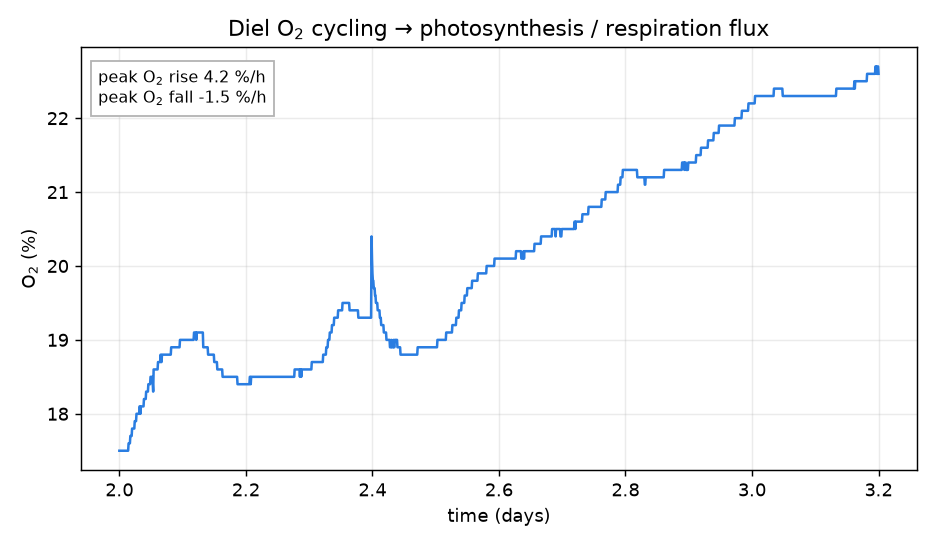
\includegraphics[width=0.72\textwidth]{F2_diel_flux.png}
\caption{\textbf{Single diel $\mathrm{O_2}$ cycle and whole-chamber flux extraction.}
Expanded $24\,\mathrm{h}$ window from the $4.8\,\mathrm{d}$ Vernier closed-chamber trace (\texttt{F2\_diel\_flux.png}) showing linear regression slopes for peak light-phase net $\mathrm{O_2}$ evolution ($+4.2\%\,\mathrm{h^{-1}}$) and dark-phase respiratory $\mathrm{O_2}$ uptake ($-1.5\%\,\mathrm{h^{-1}}$).}
\label{fig:s_diel_flux}
\end{figure}

\begin{figure}[htbp]
\centering
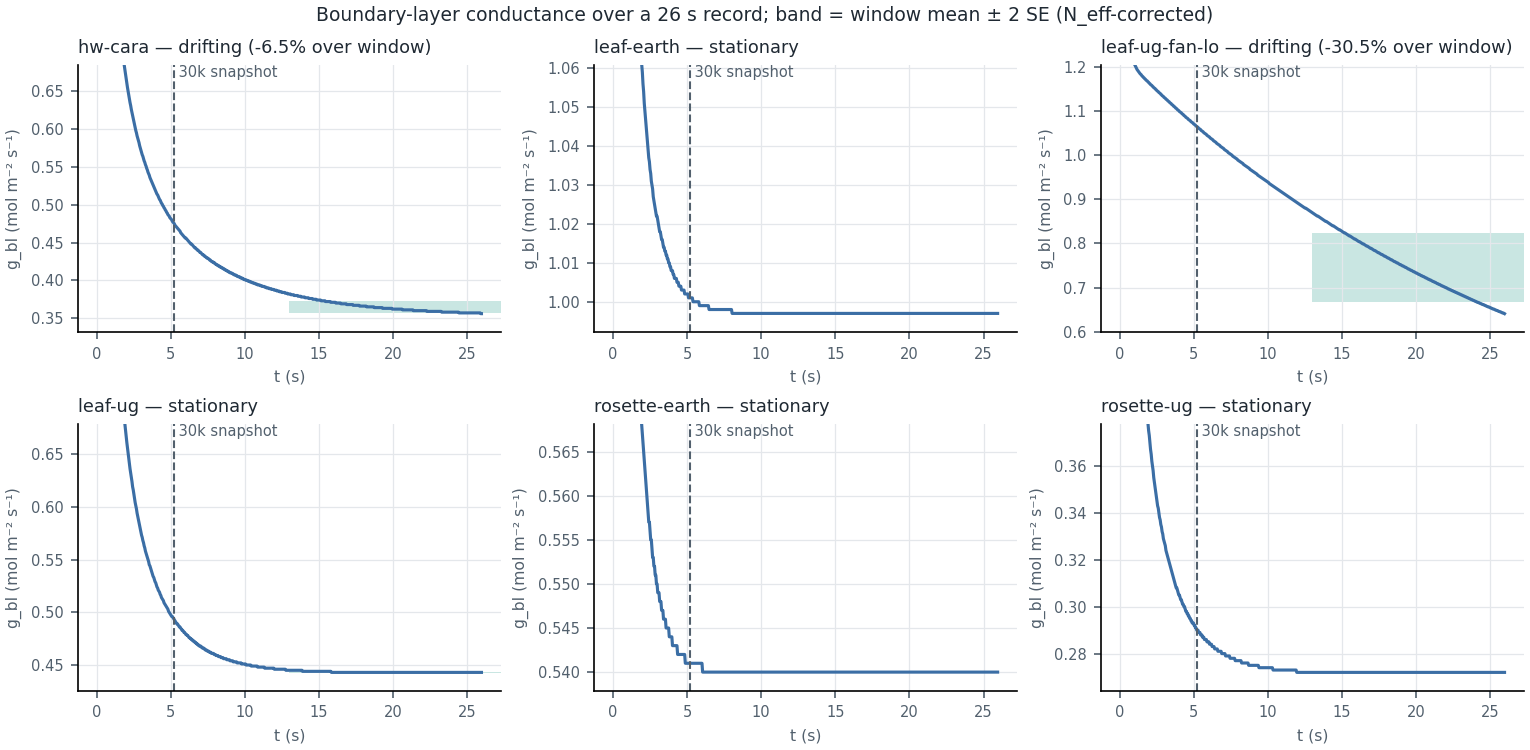
\includegraphics[width=0.48\textwidth]{F11_stationarity.png}\hfill
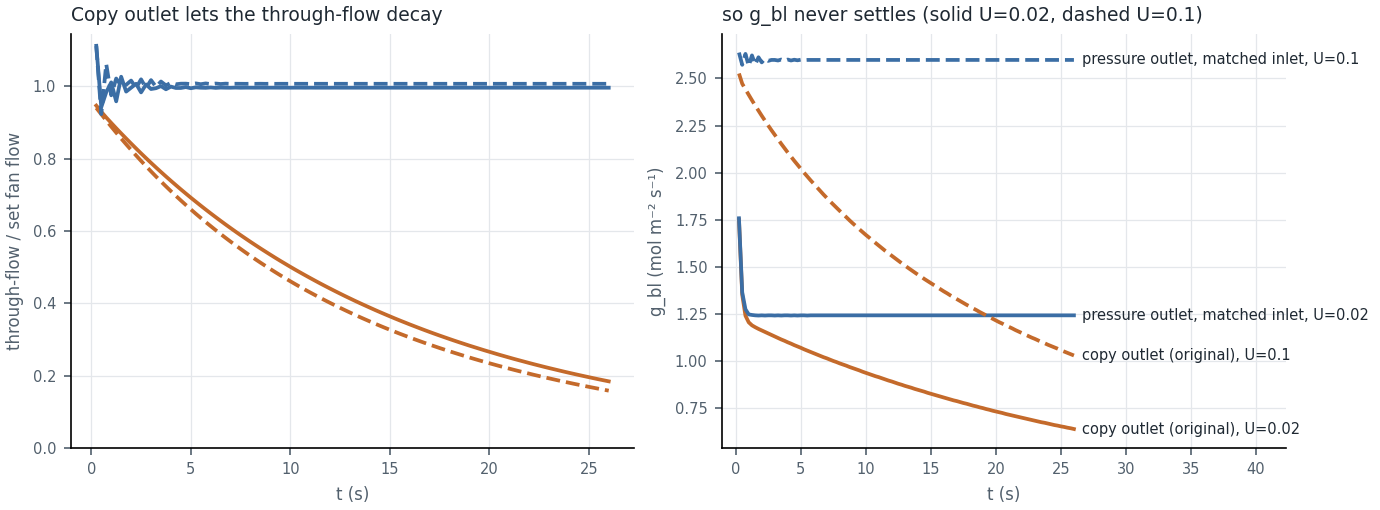
\includegraphics[width=0.48\textwidth]{F12_outlet_bc.png}
\caption{\textbf{Temporal stationarity verification and density-matched pressure-outlet validation.}
\textbf{a}, Time evolution of boundary-layer conductance $g_{bl}(t)$ over $26\,\mathrm{s}$ ($150\,\mathrm{k}$ steps; \texttt{F11\_stationarity.png}) across six representative scenarios. The vertical dashed line marks the legacy $30\,\mathrm{k}$-step ($5.2\,\mathrm{s}$) snapshot, which caught the $0\,g$ pure-diffusion runs prior to full relaxation.
\textbf{b}, Forced-airflow outlet throughput ($Q_{\mathrm{out}}/Q_{\mathrm{set}}$) and $g_{bl}(t)$ comparing the legacy zero-gradient copy outlet against the pressure-pinned outlet ($\rho=1$) paired with a density-matched velocity inlet (\texttt{F12\_outlet\_bc.png}), which delivers $99.6\text{--}100.9\%$ of the set flow.}
\label{fig:s_stationarity_outlet}
\end{figure}

\begin{figure}[htbp]
\centering
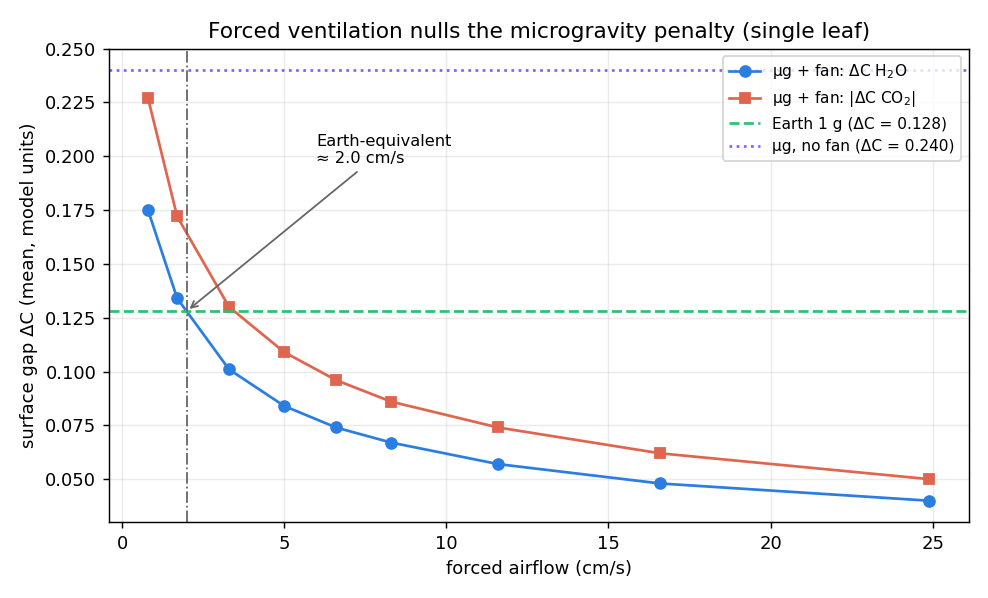
\includegraphics[width=0.48\textwidth]{F6_forced_airflow.png}\hfill
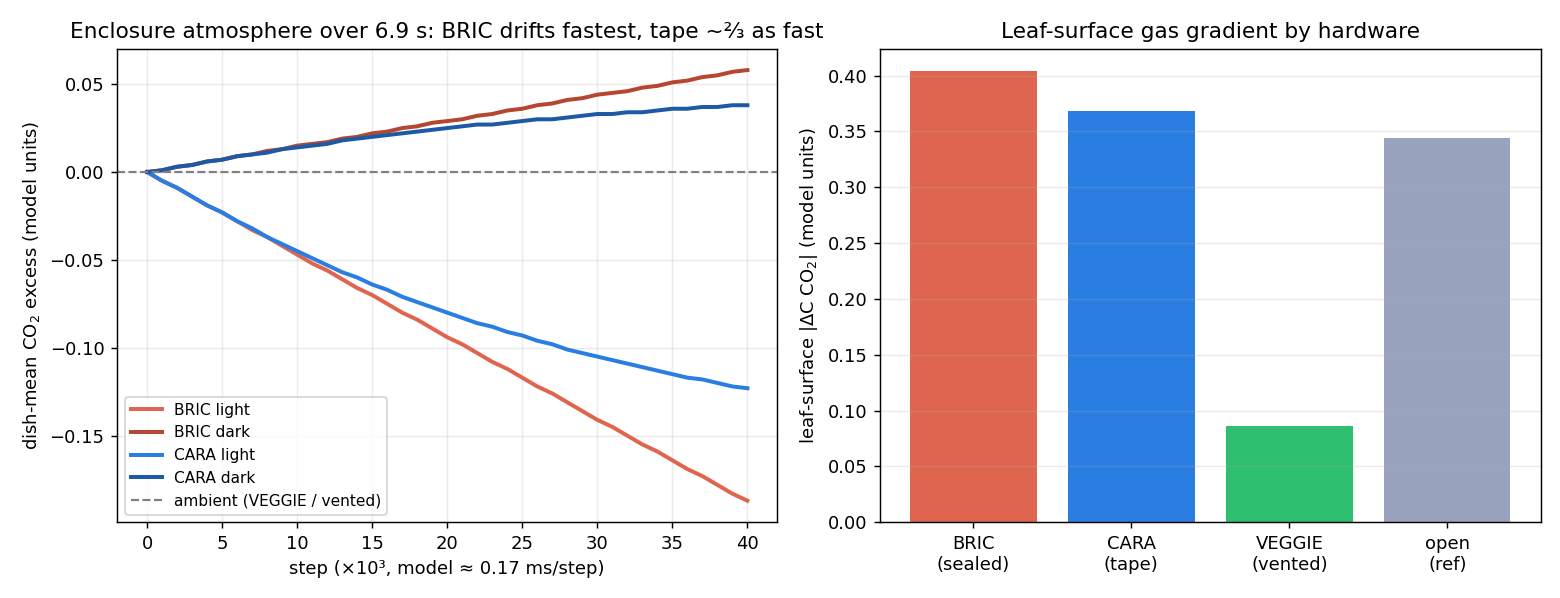
\includegraphics[width=0.48\textwidth]{F7_hardware_compare.png}
\caption{\textbf{Single-leaf forced-airflow sweep and spaceflight hardware enclosure comparison.}
\textbf{a}, Steady-state surface $\mathrm{H_2O}$ and $|\mathrm{CO_2}|$ concentration gaps versus fan speed for an isolated microgravity leaf (\texttt{F6\_forced\_airflow.png}), crossing the $1\,g$ free-convection reference at $\approx 2.0\text{--}2.1\,\cmsu$.
\textbf{b}, Short-window ($6.9\,\mathrm{s}$) lattice-Boltzmann enclosure-mean $\mathrm{CO_2}$ drift and leaf-surface concentration gradient across BRIC (sealed), CARA (micropore tape), and VEGGIE (ventilated) boundary conditions (\texttt{F7\_hardware\_compare.png}).}
\label{fig:s_leaf_fan}
\end{figure}

\begin{figure}[htbp]
\centering
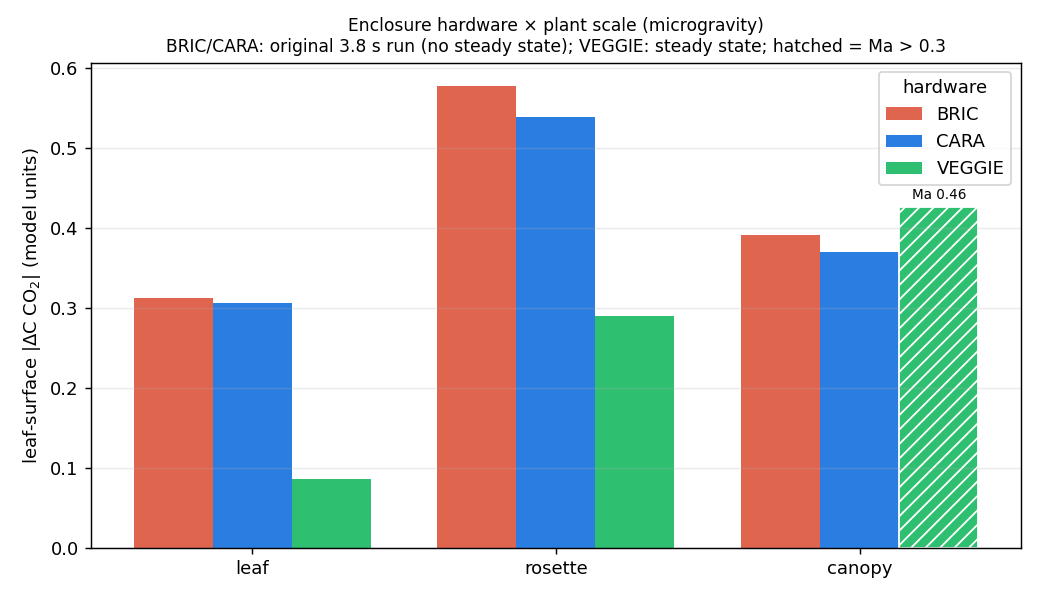
\includegraphics[width=0.48\textwidth]{F9_hardware_by_scale.png}\hfill
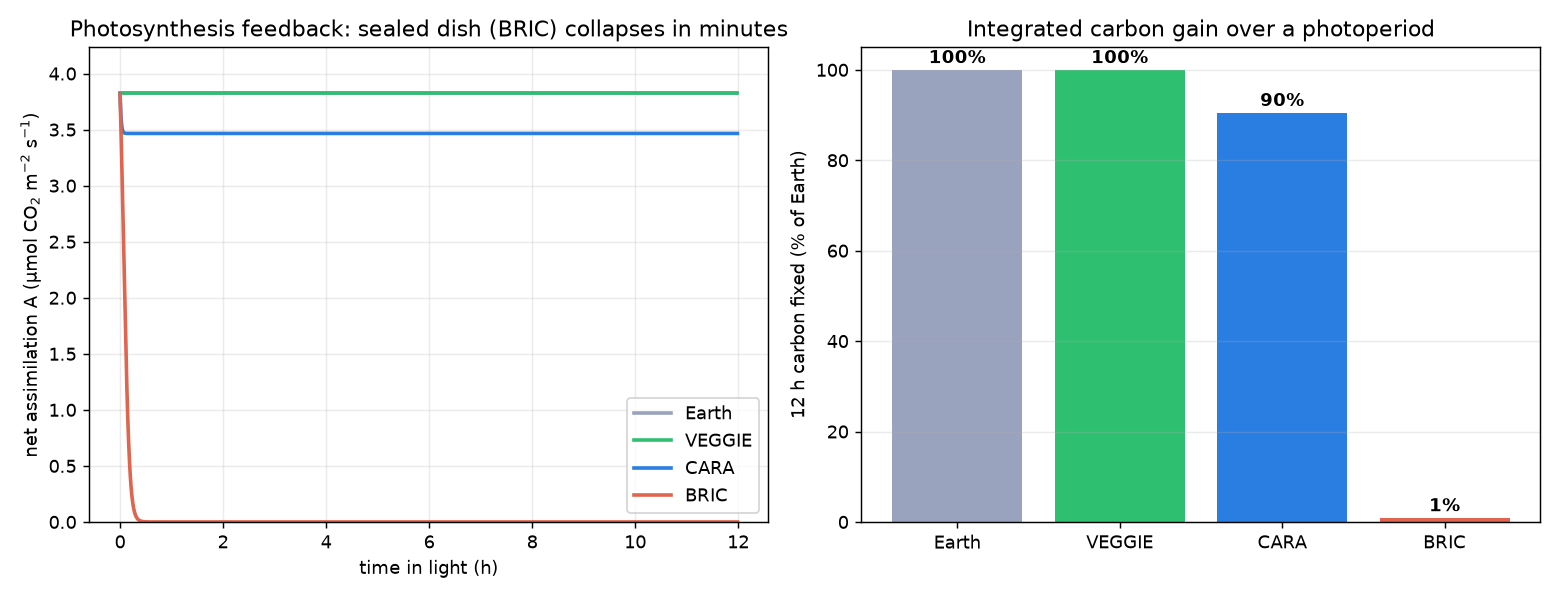
\includegraphics[width=0.48\textwidth]{F10_photosynthesis_feedback.png}
\caption{\textbf{Hardware boundary conditions across plant scales and closed-loop $\mathrm{CO_2}$-limited photosynthesis.}
\textbf{a}, Leaf-surface concentration gaps across BRIC, CARA, and VEGGIE for single leaf, rosette, and microgreen canopy scales in microgravity (\texttt{F9\_hardware\_by\_scale.png}). BRIC and CARA have nearly identical surface boundary layers at every scale; one VEGGIE fan speed ($\sim 8\,\cmsu$) restores the leaf and rosette mean but exceeds the low-Mach limit in the dense canopy (hatched bar, $\mathrm{Ma}=0.46$).
\textbf{b}, Coupled 0-D enclosure mass balance and $\mathrm{CO_2}$-limited photosynthesis over a $12\,\mathrm{h}$ photoperiod (\texttt{F10\_photosynthesis\_feedback.png}), showing collapse of net assimilation within minutes in sealed BRIC ($1\%$ of Earth carbon gain) versus $90\%$ in taped CARA and $100\%$ in ventilated VEGGIE.}
\label{fig:s_hw_scale}
\end{figure}

\begin{figure}[htbp]
\centering
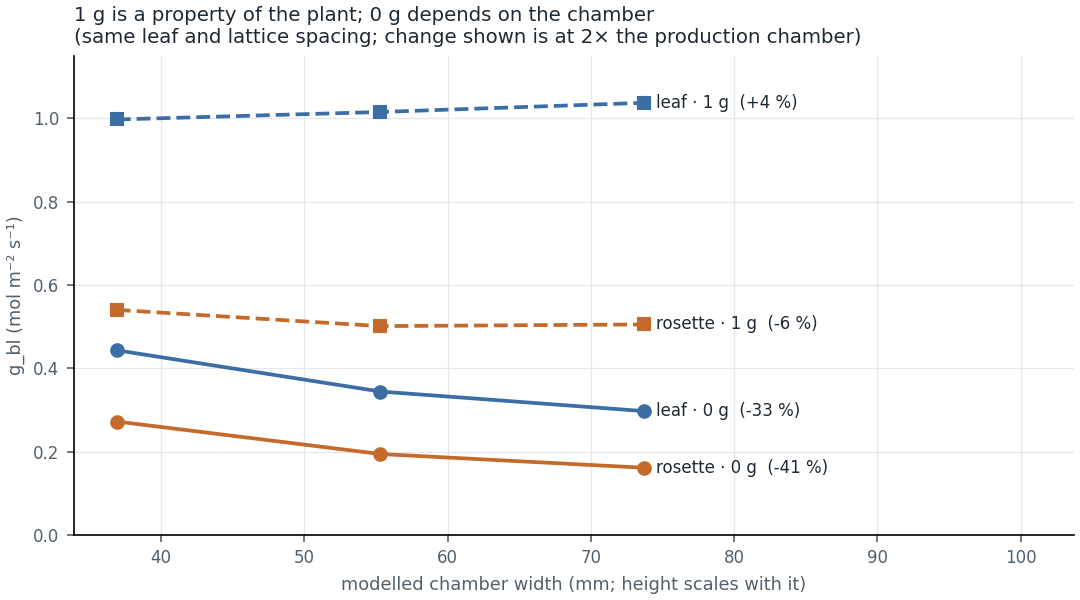
\includegraphics[width=0.78\textwidth]{F13_domain_size.png}
\caption{\textbf{Chamber domain-size sensitivity at $1\,g$ and $0\,g$.}
Boundary-layer conductance $g_{bl}$ across $1\times$, $1.5\times$, and $2\times$ domain sizes for an isolated leaf and a rosette (\texttt{F13\_domain\_size.png}, Table~\ref{tab:s_domain}). At $1\,g$, buoyant convection localizes the boundary layer and $g_{bl}$ changes by $\le 7\%$; at $0\,g$, 2-D pure diffusion spans the chamber to the ambient walls, so larger domains yield even lower $0\,g$ conductances ($-33\%$ leaf, $-41\%$ rosette at $2\times$).}
\label{fig:s_domain_size}
\end{figure}

\begin{figure}[htbp]
\centering
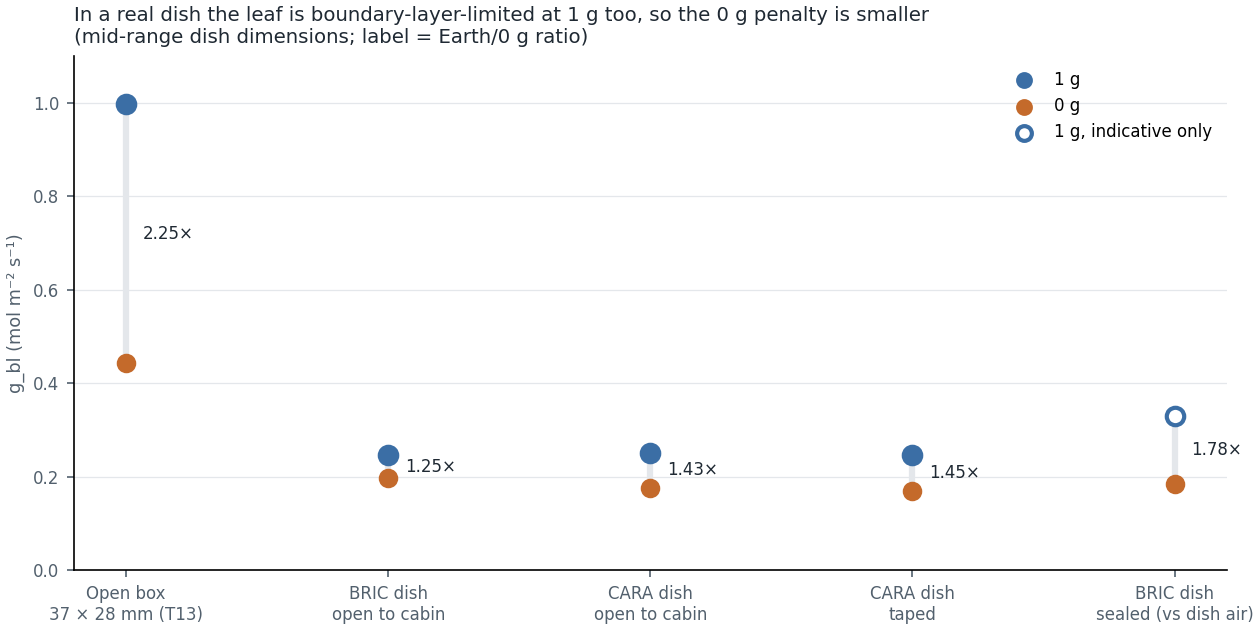
\includegraphics[width=0.78\textwidth]{F14_dish_hardware.png}
\caption{\textbf{Leaf boundary-layer conductance inside real BRIC ($60\,\mathrm{mm}$ round) and CARA ($120\,\mathrm{mm}$ square) Petri-dish cross-sections.}
Simulated $g_{bl}$ at $1\,g$ and $0\,g$ for a leaf positioned $1\,\mathrm{mm}$ above the agar floor inside actual dish geometries (\texttt{F14\_dish\_hardware.png}, Table~\ref{tab:s_real_dish}A) compared against the generic open chamber. Because the shallow $7.4\text{--}9.8\,\mathrm{mm}$ headspace restricts vertical plume development even at $1\,g$, dish $g_{bl}(1\,g)$ is $\approx 0.25\,\molms$ and the $1\,g/0\,g$ ratio inside the dish is $1.25\text{--}1.8\times$.}
\label{fig:s_real_dishes}
\end{figure}

\begin{figure}[htbp]
\centering
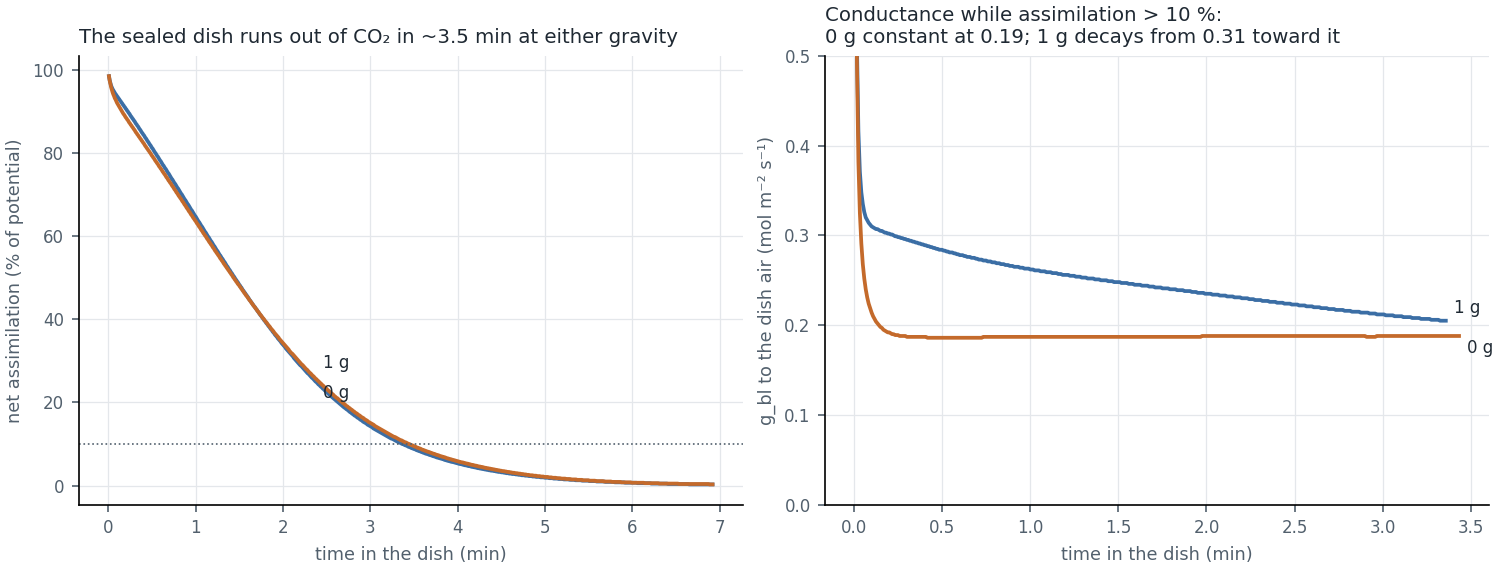
\includegraphics[width=0.49\textwidth]{F15_dish_feedback.png}\hfill
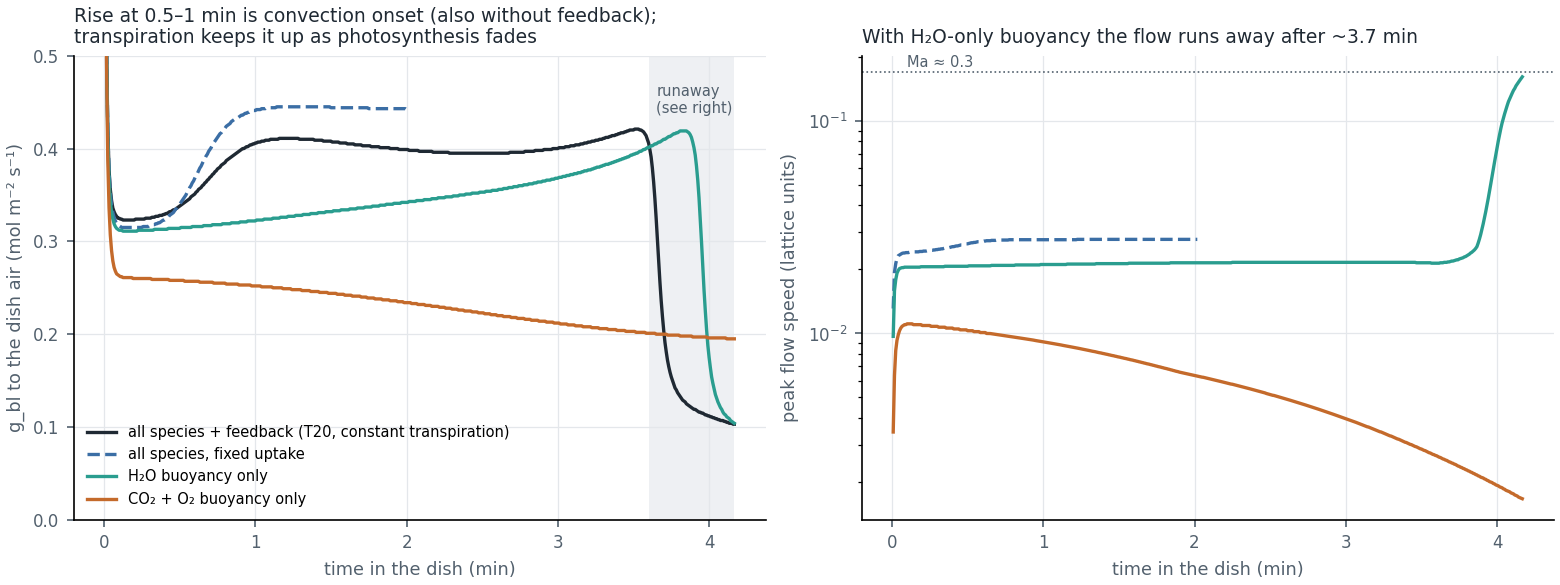
\includegraphics[width=0.49\textwidth]{F16_dish_buoyancy_diag.png}\\[0.8em]
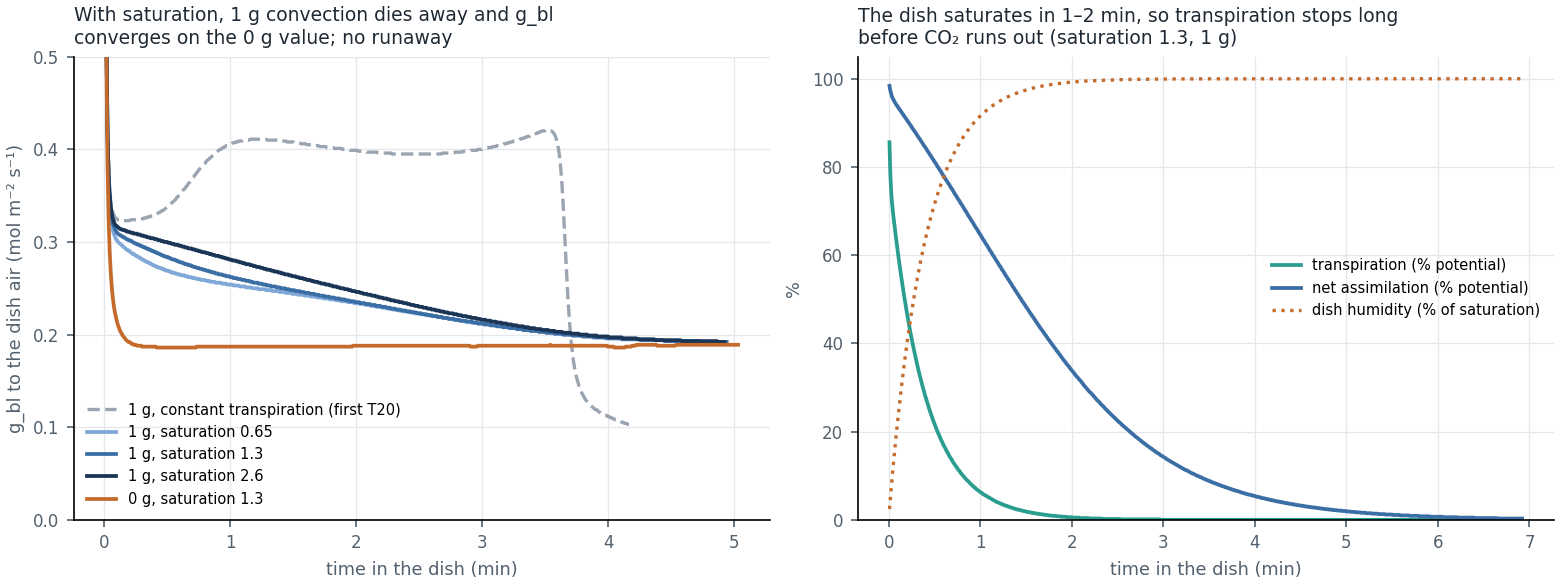
\includegraphics[width=0.72\textwidth]{F17_dish_humidity.png}
\caption{\textbf{Transient $\mathrm{CO_2}$ feedback, solutal buoyancy decomposition, and humidity-limited transpiration inside a sealed BRIC Petri dish.}
\textbf{Top left} (\texttt{F15\_dish\_feedback.png}), Net assimilation ($\%$ of potential) and leaf-to-dish $g_{bl}$ over $415\,\mathrm{s}$ in a sealed BRIC dish at $1\,g$ and $0\,g$ (\texttt{T20\_dish\_feedback.csv}): $\mathrm{CO_2}$ is exhausted in $\sim 3.5\,\mathrm{min}$ ($A < 10\%$ at $\approx 205\,\mathrm{s}$) at both gravities.
\textbf{Top right} (\texttt{F16\_dish\_buoyancy\_diag.png}), Buoyancy species decomposition at $1\,g$ (\texttt{T21\_dish\_buoyancy\_diag.csv}), showing that unbounded constant transpiration in a sealed dish causes late-time humidity runaway after $\sim 3.7\,\mathrm{min}$.
\textbf{Bottom} (\texttt{F17\_dish\_humidity.png}), Coupling transpiration to headspace humidity saturation (\texttt{T22\_dish\_humidity.csv}, \texttt{h2oSatExcess} $= 0.65, 1.3, 2.6$) eliminates the runaway: as the dish air saturates within $1\text{--}2\,\mathrm{min}$, transpiration ceases, $1\,g$ solutal convection dies out, and the $1\,g$ and $0\,g$ boundary-layer conductances converge.}
\label{fig:s_dish_feedback}
\end{figure}

\begin{figure}[htbp]
\centering
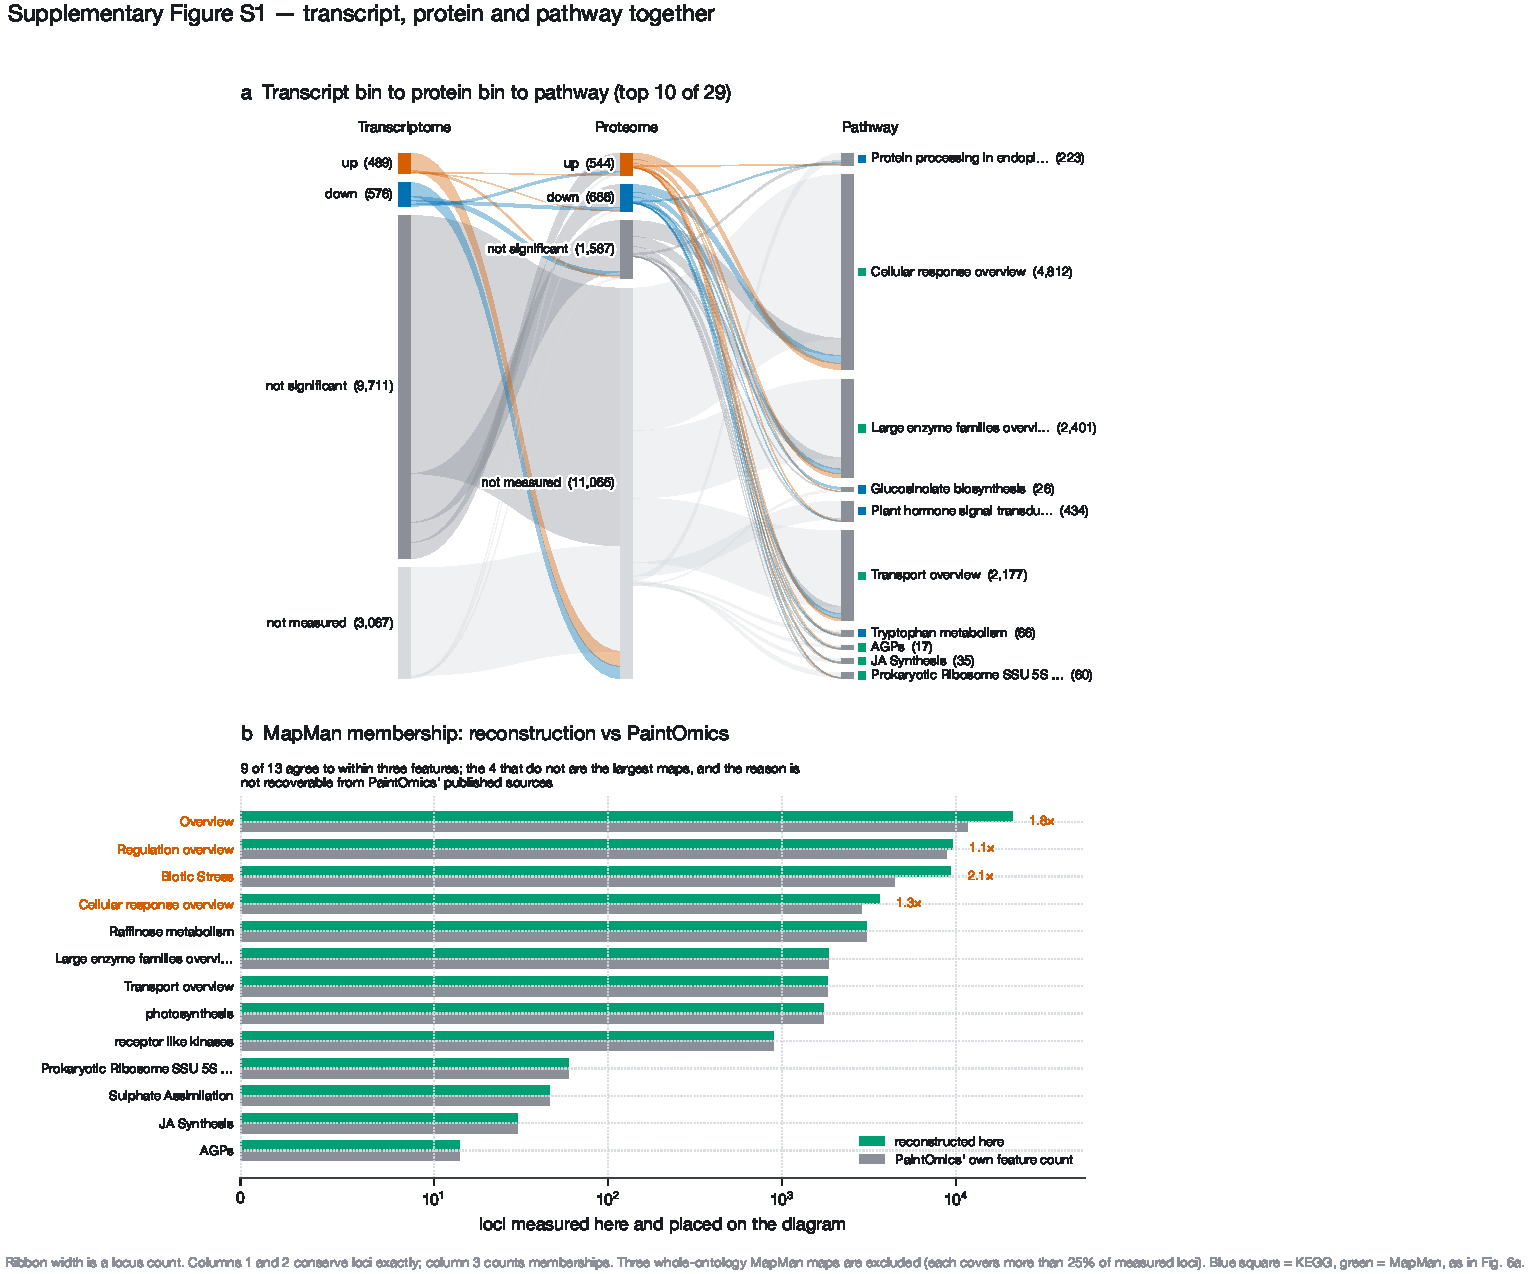
\includegraphics[width=\textwidth]{figS1_sankey.pdf}
\caption{\textbf{Multi-omics locus conservation across significant pathways and deterministic MapMan reconstruction verification.}
\textbf{a}, Sankey diagram (\texttt{figS1\_sankey.pdf}) tracing every measured \textit{Arabidopsis} locus in the 29 non-broad significant pathways ($p<0.05$) from its OSD-522 transcript bin (column 1) to its protein bin (column 2) and into the top ten enriched KEGG and MapMan pathways (column 3). Columns 1 and 2 conserve gene counts exactly ($13{,}843$ loci); column 3 counts pathway memberships ($22{,}147$).
\textbf{b}, Verification of reconstructed MapMan pathway feature counts (\texttt{scripts/mapman.py}, built from GoMapMan Araport11 mappings and MapManStore diagram XMLs) against the feature counts reported by the PaintOmics 4 server: 9 of 13 pathways agree within $\le 3$ features.}
\label{fig:s_sankey}
\end{figure}

\end{document}
